% fig-1: Three-mode single-parameter continuum over the virtual rotation centre
% (azimuth squint plane, schematic). Spec pointers: ADR 0001 sec.7 (continuum
% semantics + r0/R0 discipline) and figure-plan-review C (machine predicates).
% Predicates honoured here: no retired artefact angle of any form; the SLS cap
% is co-labelled "registered conservative value (design choice)"; r0 and R0 are
% attached to their own distances (r0 = rotation centre -> scene centre,
% R0 = aperture-centre slant range, r0/R0 = 0.254207).
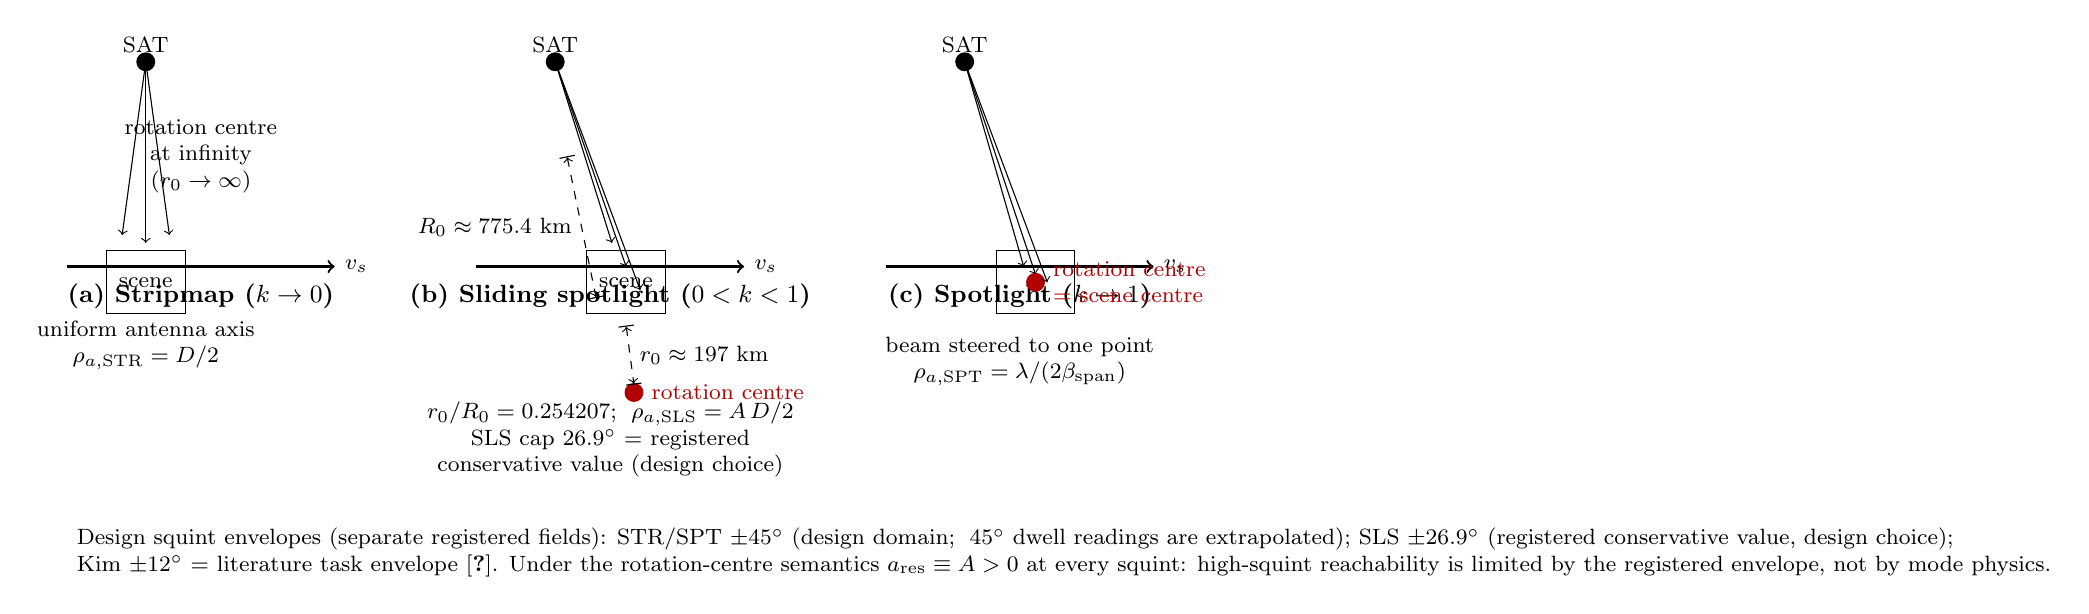
\begin{tikzpicture}[x=1mm,y=1mm,scale=1.0]
  % ------------------------------------------------------------------
  % Panel A: stripmap -- rotation centre at infinity, parallel rays
  % ------------------------------------------------------------------
  \begin{scope}[shift={(0,0)}]
    \node[anchor=north,font=\small\bfseries] at (17,-1) {(a) Stripmap ($k\to 0$)};
    % ground track
    \draw[thick,->] (0,0) -- (34,0) node[right,font=\footnotesize]{$v_s$};
    % satellite
    \fill (10,26) circle (1.2) node[above,font=\footnotesize]{SAT};
    % parallel beams (rotation centre at infinity)
    \draw[->] (10,26) -- (7,4);
    \draw[->] (10,26) -- (10,3);
    \draw[->] (10,26) -- (13,4);
    % scene
    \draw (5,-6) rectangle (15,2);
    \node[font=\footnotesize] at (10,-2) {scene};
    \node[font=\footnotesize,align=center] at (17,14) {rotation centre\\at infinity\\($r_0\to\infty$)};
    \node[font=\footnotesize,align=center] at (10,-10) {uniform antenna axis\\$\rho_{a,\mathrm{STR}}=D/2$};
  \end{scope}
  % ------------------------------------------------------------------
  % Panel B: sliding spotlight -- rotation centre beyond the scene
  % ------------------------------------------------------------------
  \begin{scope}[shift={(52,0)}]
    \node[anchor=north,font=\small\bfseries] at (17,-1) {(b) Sliding spotlight ($0<k<1$)};
    \draw[thick,->] (0,0) -- (34,0) node[right,font=\footnotesize]{$v_s$};
    \fill (10,26) circle (1.2) node[above,font=\footnotesize]{SAT};
    % rotation centre below the surface, beyond scene centre (k = 0.7973)
    \fill[red!70!black] (20,-16) circle (1.2);
    \node[font=\footnotesize,red!70!black,anchor=west] at (21,-16) {rotation centre};
    % beams through the rotation centre
    \draw[->] (10,26) -- (17.2,3);
    \draw[->] (10,26) -- (19,0);
    \draw[->] (10,26) -- (20.8,-3);
    % scene
    \draw (14,-6) rectangle (24,2);
    \node[font=\footnotesize] at (19,-2) {scene};
    % r0: rotation centre -> scene centre
    \draw[dashed,|<->|] (19,-7.5) -- (20,-15) node[midway,right,font=\footnotesize]{$r_0\approx 197~\mathrm{km}$};
    % R0: aperture-centre slant range (zero-squint reference)
    \draw[dashed,|<->|] (11.5,14) -- (15.2,-4) node[midway,left,font=\footnotesize]{$R_0\approx 775.4~\mathrm{km}$};
    \node[font=\footnotesize,align=center] at (17,-22) {$r_0/R_0=0.254207$;\; $\rho_{a,\mathrm{SLS}}=A\,D/2$\\ SLS cap $26.9^{\circ}$ = registered\\ conservative value (design choice)};
  \end{scope}
  % ------------------------------------------------------------------
  % Panel C: spotlight -- rotation centre at the target
  % ------------------------------------------------------------------
  \begin{scope}[shift={(104,0)}]
    \node[anchor=north,font=\small\bfseries] at (17,-1) {(c) Spotlight ($k\to 1$)};
    \draw[thick,->] (0,0) -- (34,0) node[right,font=\footnotesize]{$v_s$};
    \fill (10,26) circle (1.2) node[above,font=\footnotesize]{SAT};
    \fill[red!70!black] (19,-2) circle (1.2);
    \node[font=\footnotesize,red!70!black,anchor=west,align=left] at (20,-2) {rotation centre\\$=$ scene centre};
    \draw[->] (10,26) -- (17.5,0);
    \draw[->] (10,26) -- (19,-1);
    \draw[->] (10,26) -- (20.5,-2);
    \draw (14,-6) rectangle (24,2);
    \node[font=\footnotesize] at (19,-2.5) {};
    \node[font=\footnotesize,align=center] at (17,-12) {beam steered to one point\\$\rho_{a,\mathrm{SPT}}=\lambda/(2\beta_{\mathrm{span}})$};
  \end{scope}
  % ------------------------------------------------------------------
  % Envelope legend: the three squint domains, listed as separate fields
  % ------------------------------------------------------------------
  \node[anchor=north west,font=\footnotesize,align=left] at (0,-32)
    {Design squint envelopes (separate registered fields): STR/SPT $\pm 45^{\circ}$ (design domain;\; $45^{\circ}$ dwell readings are extrapolated);
     SLS $\pm 26.9^{\circ}$ (registered conservative value, design choice);\\
     Kim $\pm 12^{\circ}$ = literature task envelope \cite{kim2021optimal}. Under the rotation-centre semantics
     $a_{\mathrm{res}}\equiv A>0$ at every squint: high-squint reachability is limited by the registered envelope, not by mode physics.};
\end{tikzpicture}
